\subsection{SE-14 Buscar alumno por nombre}

\begin{figure}[htbp!]
	\begin{center}
		\fbox{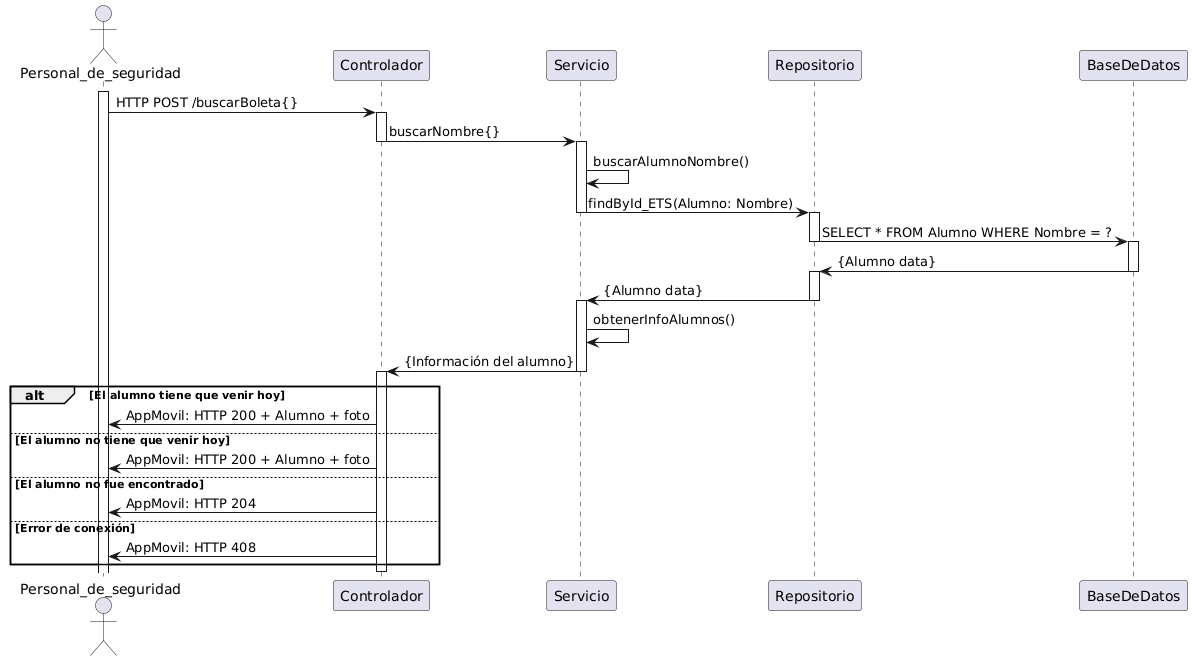
\includegraphics[width=1\textwidth]{Secuencia/CU-14.png}}
		\caption{Diagrama de secuencia del caso de uso número 14 (Buscar alumno por nombre).}
		\label{fig:Diagrama de secuencia CU-14}
	\end{center}
\end{figure}

En el diagrama de secuencia \ref{fig:Diagrama de secuencia CU-14} se describe el proceso planeado para el caso de uso \hyperlink{CU-14}{CU-14 Buscar alumno por nombre}, mostrando las interacciones que tendrá con la vista, el controlador, el servicio, el repositorio y la base de datos.

\newpage